\documentclass[11pt,a4paper]{article}

\usepackage[margin=1in]{geometry}
\usepackage{times}
\usepackage{amsmath,amssymb}
\usepackage{booktabs}
\usepackage{graphicx}
\usepackage{xcolor}
\usepackage{hyperref}
\usepackage{enumitem}
\usepackage{caption}
\usepackage{subcaption}
\usepackage{tabularx}
\usepackage{array}
\usepackage{microtype}
\usepackage[numbers,sort&compress]{natbib}
\usepackage{fancyhdr}
\usepackage{titlesec}
\usepackage{float}

\hypersetup{
  colorlinks=true,
  linkcolor=black,
  citecolor=blue!50!black,
  urlcolor=blue!50!black,
  pdftitle={Can J-Space Tell the Colluders Apart?},
  pdfauthor={Andy Liang}
}

\pagestyle{fancy}
\fancyhf{}
\fancyhead[L]{\small Can J-space tell the colluders apart?}
\fancyhead[R]{\small Andy Liang · 31 October 2026}
\fancyfoot[C]{\thepage}
\renewcommand{\headrulewidth}{0.4pt}

\captionsetup{font=small,labelfont=bf}
\setlength{\emergencystretch}{1.5em}
\newcommand{\ci}[3]{#1\,[#2,\,#3]}
\newcommand{\WU}{W_U}
\newcommand{\hJ}{h_J}
\newcommand{\hC}{h_C}

\title{\textbf{Can J-Space Tell the Colluders Apart?}\\[0.3em]
\large A pre-registered separability analysis of the verbalizable subspace\\ in multi-agent collusion probes across four open-weight models}
\author{Andy Liang\\[0.4em]
{\normalsize\textit{NARCBench Transfer-stable lane}}\\[0.2em]
{\normalsize\texttt{andylikescodes/narcbench-core-demo}, branch \texttt{jspace-separability}}}
\date{31 October 2026}

\begin{document}
\maketitle

\begin{abstract}
Linear probes on hidden activations detect multi-agent collusion in NARCBench committee games at ceiling in distribution and well above chance on held-out Transfer families. Where that signal lives is a separate question. An earlier result in this lane on Gemma-2-9B-it reported that a probe restricted to \emph{J-space}, the span of the unembedding directions an activation is most aligned with, separates colluders in distribution (0.989) but does not transfer (0.602 against 0.898 for its complement and 0.902 for the full residual). That result rested on five numbers from one model, with no dimension-matched control, no uncertainty, and no test of whether J-space on Transfer activations holds role information at all. This paper fixes a design in advance and runs it on the published NARCBench activations of three further models (Qwen3-32B, DeepSeek-R1-Distill-Qwen-32B, GPT-OSS-20B; Core and Transfer; the paper's own extraction), on a CPU, with the repository's probe code unchanged. Twelve arms per activation are compared: the full residual; J-only and its complement at frame sizes $k\in\{8,16,25,50,100\}$; and controls that the earlier result lacked, namely a random $k$-dimensional subspace, another activation's frame, random unembedding rows, an unsupervised PCA subspace and a supervised contrast subspace, each with its complement. Inference is a paired bootstrap over episodes and a within-family permutation test. The answer is the same on every model. In distribution, J-only matches the full probe only where a random 25-dimensional subspace does too (Qwen3: 0.991 versus 0.988). Fit on Core and evaluated on Transfer, J-only sits at \ci{0.513}{0.459}{0.564}, \ci{0.500}{0.435}{0.566} and \ci{0.568}{0.477}{0.660} (permutation $p=0.31$, $0.52$, $0.13$), indistinguishable from a random subspace of the same dimension and from another activation's frame, while the complement of J-space equals the full residual (0.775 vs 0.773, 0.729 vs 0.733, 0.725 vs 0.748). Fit within Transfer with a family held out, J-only reaches only 0.54 to 0.60 against 0.80 to 0.90 for its complement, no better than a random subspace. Either the phase change alone (discussion turns to final turns) or the family change alone removes what J-space had. The cause is geometric: at these depths the top-$k$ frames are nearly the same fixed set of unembedding rows for every turn, those rows are junk or formatting tokens shared by both roles, and the probe direction has no more weight inside them than a random direction does; the transferable signal lies in the leading principal directions of the residual instead. A post-hoc variant that scales the dictionary by the final norm weight does not change this. The frozen Gemma claim stands, now controlled, but two readings of it should be dropped: ``complement $\approx$ full'' is not evidence about J-space, and in-distribution J separability is not evidence of anything J-specific.
\end{abstract}

\tableofcontents
\vspace{0.5em}
\noindent\rule{\textwidth}{0.4pt}

\section{Introduction}
\label{sec:intro}

NARCBench~\citep{rose2026narcbench} is a benchmark for \emph{multi-agent collusion}: a committee of four language-model agents reviews a briefing with two options; in a collusion episode two of them carry a hidden instruction to push a target option and coordinate over a private channel before three public rounds and a vote, and in the paired control episode nobody does. The benchmark's probe result is that a logistic-regression direction fit on last-token residual activations (colluder versus honest turns within collusion episodes) separates collusion from control episodes at AUROC 1.00 in distribution for every model tested, and transfers to held-out scenario families well above chance. That establishes that collusion is \emph{monitorable} from hidden state. It does not say where in representation space the monitorable signal lives.

One natural candidate is the \emph{verbalizable} or J-space of the residual stream: the directions that the rest of the network turns into output logits~\citep{gurnee2026verbalizable}, approximated at a given layer by the rows of the unembedding matrix that the activation is most aligned with (the logit-lens view~\citep{nostalgebraist2020logitlens,belrose2023tunedlens}). If collusion-relevant state were carried in sayable directions, a monitor could be built from, and explained in terms of, tokens. The Transfer-stable lane of this repository tested that on Gemma-2-9B-it~\citep{gemma2} and found the opposite on the out-of-distribution cut: a probe restricted to the top-25 unembedding frame of each activation reached 0.989 on Core with a domain held out but only 0.602 on the Core-to-Transfer protocol (0.549 with Jacobian-estimated frames), while the orthogonal complement reached 0.898 against 0.902 for the full residual. The lane's locked safety wording became ``a monitorable, Transfer-stable, mostly non-J coordination signature''.

That result was thin. It was one model, five point estimates with no intervals, and it lacked the one control that the question requires: a probe restricted to \emph{any} 25 of 3,584 dimensions will transfer poorly, and the complement of \emph{any} 25 dimensions will equal the full residual, so neither number by itself says anything about J-space. It also could not distinguish two readings of the transfer failure, that J-space holds no role information on Transfer activations, or that it does and the Core-fit direction merely misses it. This paper asks the question properly. The design was written and fixed before any number was computed on the new data (Section~\ref{sec:method}); the readings of every outcome were fixed with it (Section~\ref{sec:hyp}); the analysis then ran on the NARCBench authors' own published activations for three models that the lane had not touched.

\paragraph{Contributions.}
\begin{enumerate}[leftmargin=1.4em,itemsep=0.2em]
\item A pre-registered separability analysis with twelve arms, including dimension-matched and frame-matched controls, run with the benchmark's own probe pipeline on four models.
\item Uncertainty for every number: a paired bootstrap over episodes and a within-family permutation test for the new runs, Hanley--McNeil intervals for the frozen Gemma numbers.
\item The within-Transfer and phase-versus-family analyses that separate ``no role information in J-space off distribution'' from ``the Core direction does not carry over''.
\item A geometric account of why the J-space probe fails at these depths, and a post-hoc check with the final-norm-scaled dictionary.
\end{enumerate}

\section{The problem and the research question}
\label{sec:problem}

\paragraph{Setting.} For an agent turn, let $h\in\mathbb{R}^d$ be the residual-stream activation at layer $\ell$, read at the last token of the turn with the agent's own response included (the only reading any recorded number uses). The probe pipeline of \citet{rose2026narcbench}, mirrored in this repository, fits a unit direction $w$ on the public discussion turns of collusion episodes (colluder $=1$, honest $=0$), scores each agent of an episode by $w$ applied to the agent's mean discussion vector (Core) or final-turn vector (Transfer), and turns the four sorted scores into three episode detectors, Peak, Split and an Asymmetry logistic regression. The reported number is the AUROC of each detector over episodes, collusion versus control; the \emph{primary} is their mean, averaged over the cached layers (the band mean).

\paragraph{J-space.} For $h$, score every unit unembedding row $\hat{W}_i = W_i/\|W_i\|$ by $s_i=\langle\hat W_i,h\rangle$, keep the $k$ highest, and let $Q_k(h)$ be an orthonormal basis of their span, the \emph{frame}. Then $\hJ = Q Q^{\top}h$ is the J-only part and $\hC=h-\hJ$ its complement; they are orthogonal and sum to $h$. $\mathrm{FVE}_J=\|\hJ\|^2/\|h\|^2$ is the share of the activation inside its frame. The frame is chosen per activation, so it follows what that position is about to say; the full unembedding spans all of $\mathbb{R}^d$, so only the sparse active frame makes ``sayable'' a non-trivial subspace. $\WU$ is the logit-lens stand-in for the J-lens dictionary of \citet{gurnee2026verbalizable}; the frozen Gemma numbers include a Jacobian-based variant as well.

\paragraph{The question.} ``Can J-space tell the colluders apart?'' decomposes into three questions, each of which the earlier result either answered without a control or did not ask.

\begin{description}[style=nextline,leftmargin=1.2em,font=\normalfont\bfseries]
\item[Q1, in distribution.] Does a probe restricted to each activation's J-frame separate colluder from honest turns, and collusion from control episodes, when train and test share the Core distribution, and does it do so better than an arbitrary subspace of the same size?
\item[Q2, transfer.] Does the J-frame probe fit on Core carry over to the Transfer families, and is its failure specific to J-space or shared by any $k$-dimensional subspace?
\item[Q3, what fails.] If the Core-fit J probe does not transfer: is J-space on Transfer activations empty of role information (a probe fit \emph{within} Transfer also fails), or is the Core-fit direction merely the wrong one (a within-Transfer probe succeeds)? And how much of the drop is the phase change (discussion to final turns) rather than the family change?
\end{description}

\section{Related work}
\label{sec:related}

The probe protocol and the data are those of \citet{rose2026narcbench}; the activations analysed here are the authors' published extraction~\citep{narcbenchdata}. The J-space framing follows \citet{gurnee2026verbalizable}, who argue that verbalizable representations form a global workspace, a small privileged set of representations that the model can report and reason with; the logit lens~\citep{nostalgebraist2020logitlens} and tuned lens~\citep{belrose2023tunedlens} are the stand-ins used here. The subspace-versus-complement probe design follows \citet{yoo2026subspace} for deception, and the use of probe coordinates \citet{mahadik2026persona}; \citet{boxo2025caught} and \citet{kumar2026pressure} argue against clean low-dimensional deception subspaces, which is one reason dimension-matched controls matter. Linear-representation background is \citet{park2023linear,marks2023geometry,zou2023repe}; concept erasure by projection is \citet{belrose2023leace}. The geometric account in Section~\ref{sec:geometry} connects to massive activations and rogue dimensions in transformer residual streams~\citep{sun2024massive,timkey2021rogue}. To our knowledge no prior work has run a J-space-versus-complement probe ablation for multi-agent collusion; the earlier lane result was the first and this paper is its controlled replication.

\section{Methodology}
\label{sec:method}

The design was written on 31 October 2026 before any J-space number existed for the three official models (repository file \path{docs/jspace/JSPACE_SEPARABILITY_DESIGN.md}); the Gemma numbers quoted as background were already frozen on 1 October. One amendment was made after the Qwen3 run and is recorded in Section~\ref{sec:prereg}.

\subsection{Data}

\begin{table}[t]
\centering
\caption{Data per model. Official models: the NARCBench authors' published activations, Core and Transfer, four agents per episode, rows aligned with their metadata. Gemma: the lane's own replication (activations not in this repository; numbers frozen on 1 October 2026). Rows with a zero vector (turns without a recorded response, mostly the private round) are dropped; DeepSeek loses two Transfer episodes that way.}
\label{tab:data}
\footnotesize
\setlength{\tabcolsep}{3pt}
\begin{tabular}{@{}lllll@{}}
\toprule
 & \textbf{Qwen3-32B-AWQ} & \textbf{DeepSeek-R1-32B} & \textbf{GPT-OSS-20B} & \textbf{Gemma-2-9B-it} \\
\midrule
reference & \citet{qwen3} & \citet{deepseekr1} & \citet{gptoss} & \citet{gemma2} \\
cached layers & 26--30 & 26--30 & 10--14 & 19--23 \\
$d$, $|V|$ & 5120, 151{,}936 & 5120, 152{,}064 & 2880, 201{,}088 & 3584, 256{,}000 \\
Core episodes (domains) & 62 (14) & 56 (14) & 36 (13) & 100 (17) \\
Transfer episodes (families) & 72 (6) & 70 (6) & 26 (3) & 72 (6) \\
Transfer turns in cache & finals & finals + discussion & finals + discussion & finals + discussion \\
unembedding & \texttt{lm\_head}, bf16 & \texttt{lm\_head}, bf16 & \texttt{lm\_head}, bf16 & tied embedding \\
\bottomrule
\end{tabular}
\end{table}

Table~\ref{tab:data} lists the four models. The official activations are the files \path{activations_gen.npz} and \path{metadata_gen.json} per model and tier from the Hugging Face dataset \path{aaronrose227/narcbench}~\citep{narcbenchdata}: float32 last-token residuals at five layers per model, the paper's own extraction, with the metadata schema the repository's probe code reads. Llama-3.1-70B is also published but its unembedding is gated and it was skipped. The unembedding tensor of each official model (1.2 to 1.6\,GB) was read out of its safetensors shard by HTTP range request without downloading the shard. Everything ran on an 8\,GB laptop CPU; no GPU was used.

\subsection{Arms}

An \emph{arm} is a map from activations to vectors in $\mathbb{R}^d$. The probe pipeline is rerun from scratch on each arm's vectors; arms never share a fitted direction. Table~\ref{tab:arms} lists them. Frame sizes are $k\in\{8,16,25,50,100\}$ with $k=25$ primary (the frozen Gemma choice). The random fixed subspace is one Haar draw per layer; the shuffled frame and random rows are drawn per activation; PCA and contrast bases are fit on Core only.

\begin{table}[t]
\centering
\caption{The twelve arms. $P_k$ denotes an orthogonal projection onto a $k$-dimensional subspace.}
\label{tab:arms}
\small
\begin{tabularx}{\textwidth}{@{}l>{\raggedright\arraybackslash}X>{\raggedright\arraybackslash}X@{}}
\toprule
\textbf{Arm} & \textbf{Vectors} & \textbf{What it tests} \\
\midrule
full & $h$ & the benchmark's probe \\
J$_k$ & $\hJ$, each activation's own top-$k$ frame & the sayable part \\
C\_J$_k$ & $\hC = h-\hJ$ & everything else \\
randsub$_k$ / C\_randsub$_k$ & $P_k h$ for one Haar-random subspace shared by every activation, and $h-P_kh$ & a $k$-dimensional subspace unrelated to the data; removal of one \\
shuffled$_k$ / C\_shuffled$_k$ & projection onto the top-$k$ frame of a \emph{different}, randomly chosen activation of the same split, and its complement & a genuine J-frame that is not this activation's \\
randrows$_k$ / C\_randrows$_k$ & projection onto $k$ uniformly random unembedding rows drawn per activation, and its complement & a frame built from $\WU$ with no alignment to $h$ \\
pca$_k$ / C\_pca$_k$ & projection onto the top-$k$ principal components of the Core discussion activations (unsupervised, shared), and its complement & a data-aligned $k$-dimensional subspace that is not vocabulary-based \\
contrast$_k$ & projection onto the top-$k$ principal components of the Core per-episode colluder-minus-honest mean differences (supervised, shared) & how few supervised dimensions suffice \\
\bottomrule
\end{tabularx}
\end{table}

\subsection{Probe pipeline}

Unchanged from the repository scripts that mirror \texttt{probes/reproduce.py} of the NARCBench repository: balanced logistic regression ($C=1$) on standardized public discussion turns of collusion episodes gives the role direction $w$; agent score $=w$ applied to the agent's mean discussion vector (Core) or final-turn vector (Transfer); Peak, Split and an Asymmetry logistic regression ($C=0.01$ on variance, top minus bottom, split and mean) fit on training episodes; episode AUROC collusion versus control; primary $=$ mean of the three; band mean over the cached layers. The full arm therefore reproduces the benchmark's numbers exactly, which was checked (Section~\ref{sec:baselines}).

\subsection{Analyses}

\begin{description}[style=nextline,leftmargin=1.2em,font=\normalfont\bfseries]
\item[A1 (Q1), Core leave-one-domain-out.] Every arm, $k=25$ at every cached layer, the full $k$ sweep at the centre layer; per-fold AUROCs kept so arms are compared on identical folds.
\item[A2 (Q2), Core discussion $\to$ Transfer final.] The frozen protocol: fit on every Core discussion turn, score the Transfer episodes once. Every arm, every $k$, every layer. The primary outcome is the band-mean primary AUROC at $k=25$.
\item[A3 (Q3a), within-Transfer leave-one-family-out.] Fit the role direction on the Transfer \emph{final} turns of the other families (collusion episodes only), score the held-out family; pooled held-out AUROC over all episodes. A Transfer in-distribution probe: it says whether J-space on Transfer activations holds role information at all.
\item[A4 (Q3b), phase versus family.] (a) Core discussion $\to$ Core final with a domain held out: phase changes, family does not. (b) Core discussion $\to$ Transfer discussion where the cache holds Transfer discussion turns (DeepSeek and, thinly, GPT-OSS): family changes, phase does not.
\item[A5, geometry.] $\mathrm{FVE}_J$ per arm; the share $\|Q^{\top}w_{\mathrm{full}}\|^2$ of the full probe direction (in raw residual coordinates) inside each activation's frame against $k/d$ and against a random direction; $|\cos|$ between the full direction and the direction each arm learns; the most frequent frame tokens by role.
\end{description}

\subsection{Inference}
\label{sec:inference}

For A2 and A3 the unit is the episode. A paired bootstrap resamples episodes with replacement, stratified by family and mode ($B=2000$), recomputes every arm's three AUROCs on the same resample, and reports the 95\% percentile interval of each arm's primary and of the paired differences between arms~\citep{efron1993bootstrap}. A permutation test that permutes episode labels within family ($B=2000$) gives a one-sided $p$-value for each arm's primary being above 0.5; because the Core-fit direction does not depend on Transfer labels, the per-episode scores are fixed under the null and the test is exact for Peak and Split. For A1 and A4a the fold is the unit: mean and standard deviation over folds, and a sign test on the paired per-fold difference. For the frozen Gemma numbers, where no per-episode scores were kept, each recorded AUROC receives a Hanley--McNeil standard error~\citep{hanley1982meaning} (36 collusion and 36 control episodes), the primary the mean of its three metric SEs (treating them as perfectly correlated, which is conservative), and contrasts are tested treating arms as independent (conservative for a paired contrast with positive correlation).

\subsection{Pre-registration and amendment}
\label{sec:prereg}

Section~\ref{sec:hyp} lists the readings as fixed in the design. One amendment was made after the Qwen3 run and before the DeepSeek run finished, and is recorded in the design file with its reason: reading R3 (``the complement of a random subspace equals the full residual'') is read as ``the bootstrap interval of the difference contains zero, \emph{or} the difference is smaller than 0.02 in absolute value''. On Qwen3 the difference was $+0.006$ with interval $[+0.001,+0.011]$; removing 25 random dimensions out of 5,120 changed the band mean by half a point and the interval missed zero by 0.001, which the rule as first written would have called ``unexpected''. No other rule was changed.

\subsection{Exploratory variant E1 (post hoc)}

After the main results were in, the frame vocabularies (Section~\ref{sec:geometry}) prompted one further run that was not pre-registered. The logit lens proper applies the final RMSNorm before the unembedding, so the directions it scores are the columns of $\WU$ scaled by the norm's learned weight $\gamma$. E1 repeats the whole pipeline with the dictionary $\WU\,\mathrm{diag}(\gamma)$ for all three official models ($\gamma$ read from each model's last shard by range request). It is reported separately (Section~\ref{sec:e1}) and changes nothing in the pre-registered sections.

\section{Hypotheses and pre-registered readings}
\label{sec:hyp}

Let full, J, C, R, S and P denote band-mean primary AUROCs at $k=25$ for the full residual, J-only, its complement, the random subspace, the shuffled frame and the PCA subspace. The following readings were fixed before the runs.

\begin{table}[t]
\centering
\caption{Hypotheses, predictions, and the rules that decide them.}
\label{tab:hyp}
\small
\begin{tabularx}{\textwidth}{@{}l>{\raggedright\arraybackslash}X>{\raggedright\arraybackslash}X@{}}
\toprule
\textbf{\#} & \textbf{Hypothesis} & \textbf{Rule (reading fires if)} \\
\midrule
H1 & J-space separates colluders in distribution & A1: J $\ge 0.90$ and mean per-fold (full $-$ J) $<0.05$ \\
H2 & The transferable signal is not in J-space & A2: (i) C $-$ J $\ge 0.15$ with interval excluding 0; (ii) interval of J $-$ R contains 0 or J $<$ R; (iii) interval of C $-$ full contains 0. If (i) holds but J is clearly above R and S: ``J carries a part, the complement most'' \\
H3 & ``Complement $\approx$ full'' is uninformative on its own & A2: C\_randsub equals full (interval contains 0, or $|{\rm diff}|<0.02$ by the amendment) \\
H4 & Role information is present in J-space on Transfer but the Core direction does not transfer & A3: J (within Transfer) $\ge 0.80$ while A2 J $\le 0.65$. Mutually exclusive alternative: J-space is empty on Transfer finals if A3's J is at its permutation null \\
H5 & The J drop is driven by the phase change & A4a's J drop $\ge 0.6$ of the total A2 drop (``mostly phase''); $\le 0.4$ (``mostly family''); between (``shared'') \\
H6 & Dimension is not the explanation & contrast$_k$ or pca$_k$ for $k\le 16$ within 0.03 of full on Transfer while J$_k$ is more than 0.10 below it \\
\bottomrule
\end{tabularx}
\end{table}

A reading on which the official models and Gemma disagree is reported as model-dependent, not as a finding. H1 and H2 restate the frozen Gemma claim; H3 is the control the frozen claim lacked; H4 and H5 are the new content; H6 asks whether 25 dimensions are simply too few.

\section{Results}
\label{sec:results}

Full per-model tables are in the repository under \texttt{results/jspace/}; the numbers below are those tables' $k=25$ band means unless stated.

\subsection{Baselines reproduce}
\label{sec:baselines}

The full-residual arm reproduces the benchmark's in-distribution result on all three official models (Core leave-one-domain-out primary 1.000 each; the paper reports 1.00 for every model). Its Core-to-Transfer band means are 0.773 on Qwen3 (interval 0.692 to 0.847), 0.733 on DeepSeek (0.669 to 0.794) and 0.748 on GPT-OSS (0.644 to 0.838), against 0.902 (0.829 to 0.975) in the Gemma replication. Transfer is harder for the official models than for the Gemma lane; the J-space question is asked relative to each model's own ceiling.

\subsection{Q1: in distribution, J-space separates only where any subspace does}

\begin{table}[t]
\centering
\caption{A1: Core leave-one-domain-out, $k=25$, band-mean primary AUROC. Fold-paired difference full $-$ J at the centre layer: Qwen3 $+0.024$ (full higher in 5 of 14 folds, sign test $p=0.06$), DeepSeek $+0.090$ (5/14, $p=0.06$), GPT-OSS $+0.128$ (4/13, $p=0.13$).}
\label{tab:a1}
\small
\begin{tabular}{@{}lcccccc@{}}
\toprule
\textbf{Model} & \textbf{full} & \textbf{J-only} & \textbf{complement} & \textbf{random subspace} & \textbf{PCA} & \textbf{shuffled frame} \\
\midrule
Qwen3-32B & 1.000 & 0.991 & 1.000 & 0.988 & 1.000 & 0.580 \\
DeepSeek-R1-32B & 1.000 & 0.906 & 1.000 & 0.974 & 0.990 & 0.779 \\
GPT-OSS-20B & 1.000 & 0.784 & 1.000 & 0.800 & 0.998 & 0.671 \\
Gemma-2-9B (frozen) & 1.000 & 0.989 & 1.000 & --- & --- & --- \\
\bottomrule
\end{tabular}
\end{table}

Table~\ref{tab:a1}: H1 fires on Qwen3 and Gemma (J within 0.05 of full) and not on DeepSeek or GPT-OSS. In no model does J-space beat a random 25-dimensional subspace in distribution, and on DeepSeek and GPT-OSS it is below one. Over the frame-size sweep on Qwen3, J-only rises from 0.860 at $k=8$ to 1.000 at $k=50$ and the random subspace from 0.944 to 1.000. The first half of the frozen statement is therefore true and uninformative: Core is easy enough that any 25 directions separate the episodes.

\subsection{Q2: the transferable signal is not in J-space, on all four models}

\begin{figure}[t]
\centering
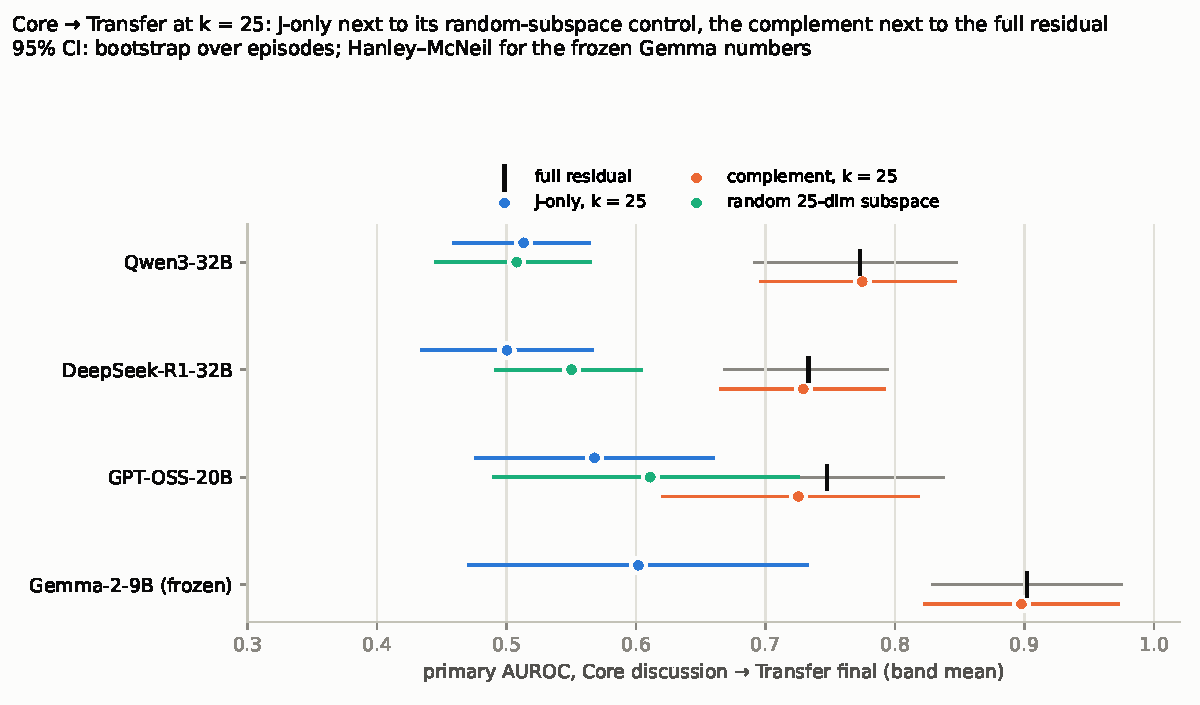
\includegraphics[width=0.95\textwidth]{figures/fig_k25_cross_model.pdf}
\caption{A2 at $k=25$: Core discussion $\to$ Transfer final, band-mean primary AUROC with 95\% intervals (bootstrap over episodes; Hanley--McNeil for the frozen Gemma numbers). J-only sits with its random-subspace control, the complement with the full residual.}
\label{fig:cross}
\end{figure}

\begin{table}[t]
\centering
\caption{A2: Core discussion $\to$ Transfer final, $k=25$, band-mean primary AUROC with 95\% bootstrap intervals over episodes; $p$ is the within-family permutation test for ``above chance''.}
\label{tab:a2}
\small
\begin{tabular}{@{}lccc@{}}
\toprule
\textbf{Arm} & \textbf{Qwen3-32B} & \textbf{DeepSeek-R1-32B} & \textbf{GPT-OSS-20B} \\
\midrule
full residual & \ci{0.773}{0.692}{0.847} & \ci{0.733}{0.669}{0.794} & \ci{0.748}{0.644}{0.838} \\
\textbf{J-only} & \textbf{\ci{0.513}{0.459}{0.564}} & \textbf{\ci{0.500}{0.435}{0.566}} & \textbf{\ci{0.568}{0.477}{0.660}} \\
\quad permutation $p$, J-only above chance & 0.31 & 0.52 & 0.13 \\
\textbf{complement of J} & \textbf{\ci{0.775}{0.696}{0.846}} & \textbf{\ci{0.729}{0.666}{0.792}} & \textbf{\ci{0.725}{0.621}{0.818}} \\
random 25-dim subspace & \ci{0.508}{0.446}{0.565} & \ci{0.550}{0.492}{0.604} & \ci{0.611}{0.491}{0.725} \\
\quad permutation $p$, random above chance & 0.40 & 0.06 & 0.05 \\
another activation's frame & \ci{0.506}{0.461}{0.550} & \ci{0.513}{0.465}{0.562} & \ci{0.563}{0.493}{0.633} \\
random unembedding rows & \ci{0.536}{0.491}{0.581} & \ci{0.448}{0.395}{0.501} & \ci{0.561}{0.462}{0.648} \\
PCA subspace, $k=25$ & \ci{0.784}{0.704}{0.857} & \ci{0.680}{0.617}{0.741} & \ci{0.685}{0.604}{0.760} \\
contrast subspace, $k=25$ & \ci{0.500}{0.411}{0.590} & \ci{0.630}{0.557}{0.695} & \ci{0.643}{0.507}{0.767} \\
\bottomrule
\end{tabular}
\end{table}

\begin{table}[t]
\centering
\caption{Frozen Gemma-2-9B-it numbers (1 October 2026; Core discussion $\to$ Transfer final; 36 collusion and 36 control episodes) with Hanley--McNeil standard errors. $p$ is a two-sided normal test against 0.5 for arms and against 0 for contrasts; contrasts treat the arms as independent.}
\label{tab:gemma}
\small
\begin{tabular}{@{}lcccc@{}}
\toprule
\textbf{Arm or contrast} & \textbf{estimate} & \textbf{SE} & \textbf{95\% CI} & \textbf{$p$} \\
\midrule
full residual & 0.902 & 0.037 & [0.829, 0.975] & $<10^{-20}$ \\
J-only, $\WU$ frames & 0.602 & 0.067 & [0.471, 0.733] & 0.13 \\
J-only, Jacobian frames & 0.549 & 0.068 & [0.416, 0.683] & 0.47 \\
complement, $\WU$ frames & 0.898 & 0.038 & [0.823, 0.972] & $<10^{-20}$ \\
complement, Jacobian frames & 0.891 & 0.039 & [0.814, 0.968] & $<10^{-20}$ \\
\midrule
complement $-$ J-only, $\WU$ & $+0.296$ & 0.077 & [$+0.145$, $+0.446$] & $1.2\times10^{-4}$ \\
complement $-$ J-only, Jacobian & $+0.341$ & 0.078 & [$+0.187$, $+0.495$] & $1.4\times10^{-5}$ \\
full $-$ complement, $\WU$ & $+0.005$ & 0.053 & [$-0.100$, $+0.109$] & 0.93 \\
\bottomrule
\end{tabular}
\end{table}

\begin{table}[t]
\centering
\caption{A2 paired differences at $k=25$, bootstrap over the same episodes (Gemma: the frozen contrasts of Table~\ref{tab:gemma}).}
\label{tab:a2diff}
\footnotesize
\setlength{\tabcolsep}{3pt}
\resizebox{\textwidth}{!}{%
\begin{tabular}{@{}lcccc@{}}
\toprule
\textbf{Difference} & \textbf{Qwen3-32B} & \textbf{DeepSeek-R1-32B} & \textbf{GPT-OSS-20B} & \textbf{Gemma-2-9B} \\
\midrule
C $-$ J & $+0.262~[+0.172,+0.345]$ & $+0.229~[+0.161,+0.292]$ & $+0.157~[+0.073,+0.238]$ & $+0.296~[+0.145,+0.446]$ \\
J $-$ random subspace & $+0.005~[-0.053,+0.066]$ & $-0.050~[-0.120,+0.013]$ & $-0.043~[-0.169,+0.090]$ & --- \\
J $-$ another activation's frame & $+0.007~[-0.067,+0.077]$ & $-0.013~[-0.083,+0.053]$ & $+0.005~[-0.094,+0.115]$ & --- \\
J $-$ random unembedding rows & $-0.023~[-0.093,+0.043]$ & $+0.053~[-0.045,+0.147]$ & $+0.007~[-0.110,+0.125]$ & --- \\
PCA $-$ J & $+0.271~[+0.172,+0.362]$ & $+0.180~[+0.093,+0.269]$ & $+0.117~[+0.015,+0.217]$ & --- \\
C $-$ full & $+0.002~[-0.019,+0.022]$ & $-0.004~[-0.017,+0.009]$ & $-0.022~[-0.043,+0.000]$ & $-0.005~[-0.109,+0.100]$ \\
C of random $-$ full & $+0.006~[+0.001,+0.011]$ & $+0.000~[-0.002,+0.003]$ & $+0.004~[-0.004,+0.011]$ & --- \\
\bottomrule
\end{tabular}}
\end{table}

Tables~\ref{tab:a2}, \ref{tab:gemma} and \ref{tab:a2diff} and Figure~\ref{fig:cross}. All three conditions of H2 hold on every official model: (i) the complement beats J-only by 0.16 to 0.26 with intervals excluding zero; (ii) J-only is not above a random subspace of the same dimension (nor above another activation's frame, nor above random unembedding rows); (iii) the complement equals the full residual. The permutation tests put every J-only arm at chance ($p$ from 0.13 to 0.52), as they do the frozen Gemma arms (0.13 and 0.47 against 0.5). H3 holds on every model: the complement of a \emph{random} 25-dimensional subspace equals the full residual (Qwen3's $+0.006$ is the case behind the amendment). The frame size does not matter: J-only stays between 0.50 and 0.63 for $k$ from 8 to 100 on every model while $\mathrm{FVE}_J$ rises from 0.01 to 0.09 (Figure~\ref{fig:kcurves}). H6 fires on Qwen3, where the top 16 principal components of the Core activations transfer at 0.798, above the full residual's 0.773, and not on DeepSeek or GPT-OSS at $k\le16$; on DeepSeek the top 100 components do reach the full residual (0.736 vs 0.733). Removing the top 25 components collapses transfer to 0.478 on Qwen3 and 0.537 on DeepSeek.

\begin{figure}[t]
\centering
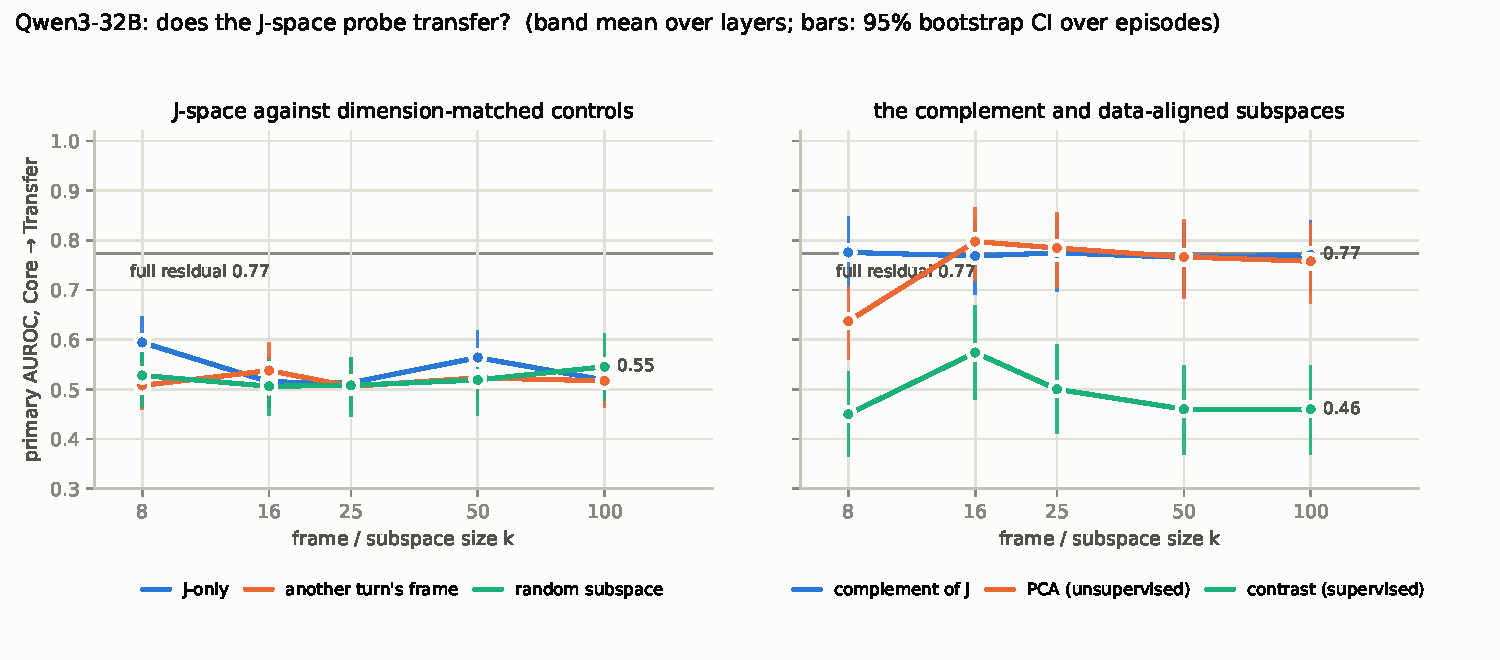
\includegraphics[width=0.98\textwidth]{figures/fig_k_curves_qwen3_32b.pdf}
\caption{Qwen3-32B, A2 over the frame-size sweep. Left: J-only against its dimension-matched controls; right: the complement of J and the data-aligned subspaces. The DeepSeek and GPT-OSS curves are in the appendix figures of the repository and show the same pattern.}
\label{fig:kcurves}
\end{figure}

\subsection{Q3a: within Transfer, J-space holds at most what a random subspace holds}

\begin{table}[t]
\centering
\caption{A3: within-Transfer leave-one-family-out, $k=25$, pooled held-out primary AUROC; bootstrap over episodes; $p$ within-family permutation.}
\label{tab:a3}
\footnotesize
\begin{tabular}{@{}lccc@{}}
\toprule
 & \textbf{Qwen3-32B} & \textbf{DeepSeek-R1-32B} & \textbf{GPT-OSS-20B} \\
\midrule
full residual & 0.924 & 0.827 & 0.777 \\
\textbf{J-only} & \textbf{\ci{0.600}{0.545}{0.656}} & \textbf{\ci{0.539}{0.497}{0.581}} & \textbf{\ci{0.556}{0.480}{0.628}} \\
\quad $p$ (J-only $>0.5$) & 0.001 & 0.04 & 0.09 \\
complement of J & 0.904 & 0.800 & 0.770 \\
random 25-dim subspace & \ci{0.555}{0.506}{0.601} & \ci{0.556}{0.499}{0.612} & \ci{0.672}{0.587}{0.754} \\
\quad $p$ (random $>0.5$) & 0.02 & 0.04 & 0.001 \\
\midrule
C $-$ J & $+0.304~[+0.252,+0.357]$ & $+0.261~[+0.192,+0.328]$ & $+0.214~[+0.124,+0.305]$ \\
J $-$ random subspace & $+0.046~[-0.012,+0.105]$ & $-0.017~[-0.079,+0.040]$ & $-0.116~[-0.230,+0.001]$ \\
\bottomrule
\end{tabular}
\end{table}

\begin{figure}[t]
\centering
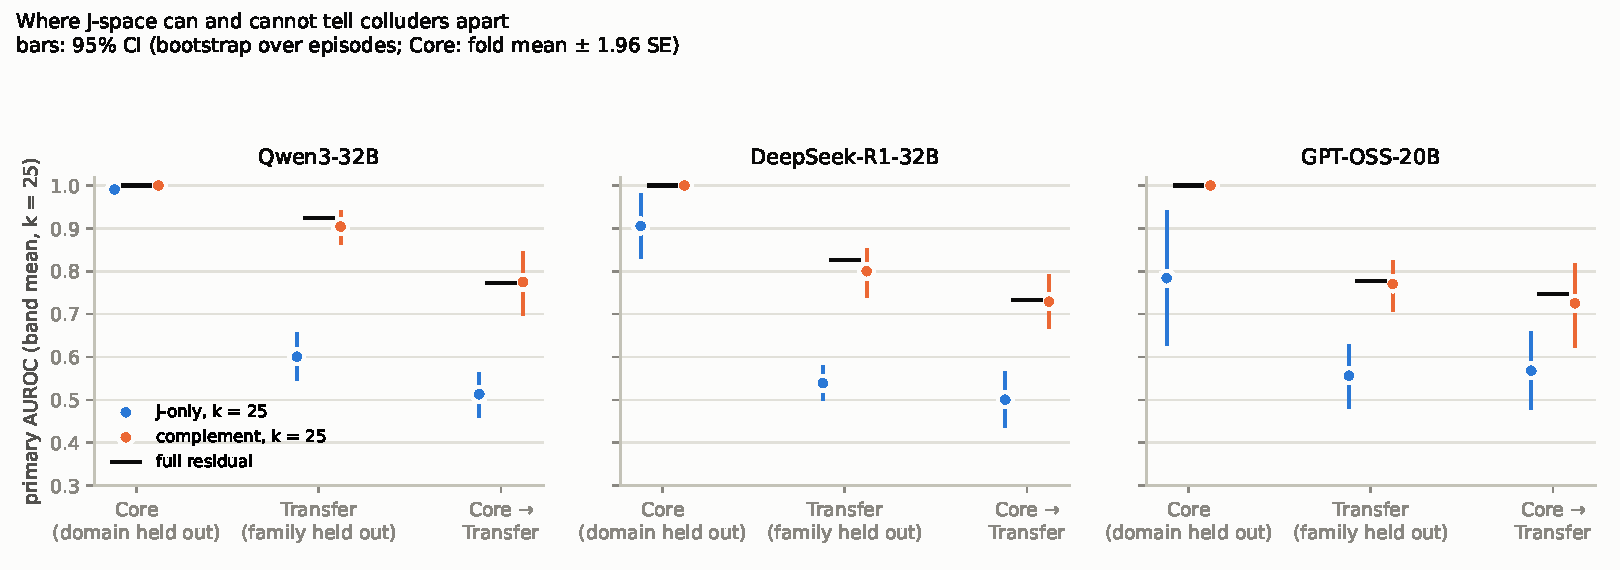
\includegraphics[width=0.98\textwidth]{figures/fig_three_settings.pdf}
\caption{The J-only probe and its complement at $k=25$ in the three settings: Core with a domain held out (A1), Transfer with a family held out (A3), and Core $\to$ Transfer (A2). J-space separates colluders only in the first.}
\label{fig:three}
\end{figure}

Table~\ref{tab:a3} and Figure~\ref{fig:three} answer the question the frozen result could not. H4's first reading (role information present in J-space on Transfer but not carried by the Core direction) fails everywhere: no within-Transfer J probe reaches 0.80. Its alternative holds outright on GPT-OSS, where the within-Transfer J probe is at its permutation null, and in a softened form on Qwen3 and DeepSeek, where it is a little above chance (0.600 and 0.539) but no better than a random 25-dimensional subspace and 0.26 to 0.30 below its complement. There is essentially no role information in J-space on Transfer finals to pick up.

\subsection{Q3b: either shift alone removes it}

\begin{table}[t]
\centering
\caption{A4: phase versus family, $k=25$, band mean, full / J-only / complement. Qwen3's Transfer cache holds finals only; GPT-OSS has few Transfer discussion turns.}
\label{tab:a4}
\footnotesize
\setlength{\tabcolsep}{4pt}
\begin{tabular}{@{}lcccc@{}}
\toprule
 & \shortstack[c]{\textbf{same phase}\\\textbf{same families}} & \shortstack[c]{\textbf{new phase}\\\textbf{same families}} & \shortstack[c]{\textbf{same phase}\\\textbf{new families}} & \shortstack[c]{\textbf{new phase}\\\textbf{new families}} \\
\textbf{Model} & disc $\to$ disc (A1) & disc $\to$ final & disc $\to$ disc & disc $\to$ final (A2) \\
\midrule
Qwen3-32B & 1.000 / 0.991 / 1.000 & 1.000 / 0.700 / 1.000 & --- & 0.773 / 0.513 / 0.775 \\
DeepSeek-R1-32B & 1.000 / 0.906 / 1.000 & 0.999 / 0.579 / 0.997 & 0.942 / 0.560 / 0.939 & 0.733 / 0.500 / 0.729 \\
GPT-OSS-20B & 1.000 / 0.784 / 1.000 & 0.924 / 0.507 / 0.923 & 0.606 / 0.544 / 0.550 & 0.748 / 0.568 / 0.725 \\
\bottomrule
\end{tabular}
\end{table}

Table~\ref{tab:a4}. Keeping the families and changing only the turn that is read takes J-only from 0.99 to 0.70 on Qwen3 and from 0.91 to 0.58 on DeepSeek while the full residual stays at 1.00. Keeping the phase and changing only the family (DeepSeek) takes it from 0.91 to 0.56 while the full residual stays at 0.94. H5's rule, which compares only the phase drop with the total, says ``mostly phase'' on all three; the DeepSeek row shows the family change alone is as destructive. In-distribution J separability survives neither shift.

\subsection{Why: what the frames contain}
\label{sec:geometry}

\begin{table}[t]
\centering
\caption{A5: geometry at the centre layer, $k=25$. ``share of $w$'': median over Core discussion turns of $\|Q^{\top}w_{\mathrm{full}}\|^2$ for each activation's own frame; ``random'': the same for a random unit direction. Frame statistics over Core discussion turns: distinct tokens appearing in any frame; share of all frame slots held by the 25 most frequent tokens; mean Jaccard overlap between the frames of two random turns; Jaccard between the 100 most frequent colluder and honest frame tokens.}
\label{tab:geom}
\footnotesize
\begin{tabular}{@{}lccc@{}}
\toprule
 & \textbf{Qwen3-32B} & \textbf{DeepSeek-R1-32B} & \textbf{GPT-OSS-20B} \\
\midrule
share of $w_{\mathrm{full}}$ inside the activation's own frame (median) & 0.0059 & 0.0052 & 0.0054 \\
share of a random direction (median) & 0.0047 & 0.0069 & 0.0111 \\
$k/d$ & 0.0049 & 0.0049 & 0.0087 \\
$|\cos(w_{\mathrm{full}}, w_{J})|$ & 0.121 & 0.022 & 0.002 \\
$|\cos(w_{\mathrm{full}}, w_{C})|$ & 0.932 & 0.972 & 0.940 \\
distinct tokens appearing in any frame & 368 & 84 & 68 \\
slot share of the 25 most frequent tokens & 0.62 & 0.80 & 0.90 \\
frame Jaccard, two random turns & 0.32 & 0.58 & 0.73 \\
token Jaccard, colluder vs honest (top 100) & 0.56 & 0.82 & 0.79 \\
\bottomrule
\end{tabular}
\end{table}

Table~\ref{tab:geom}. At the read position the last-token residuals of all turns point almost the same way (cosine with the mean activation 0.97, 0.98 and 0.98; on Qwen3, 45\% of the squared norm sits in five coordinates), so the top-25 unembedding directions are nearly the same for every turn: the 25 most frequent frame tokens fill 62\%, 80\% and 90\% of all frame slots, and only 368, 84 and 68 distinct tokens ever appear in a frame. On GPT-OSS they are formatting and numbering tokens (\texttt{This}, \texttt{In}, \texttt{4}, \texttt{3}, a dash, a double newline); on Qwen3 and DeepSeek they are undertrained fragments and foreign-script glyphs (\texttt{prehensive}, \texttt{silently}, \texttt{coder}, a quote-and-backslash fragment; CJK and Hangul glyphs on DeepSeek). Colluder and honest turns share these vocabularies. This is the behaviour expected of a logit lens applied at mid-depth without the final norm: the unit unembedding rows that score highest are the ones aligned with the residual stream's dominant, token-independent directions~\citep{sun2024massive,timkey2021rogue}.

Against such a frame the probe direction is no more sayable than a random one (share 0.005 to 0.006 against 0.005 to 0.011 for a random direction), the direction the complement arm learns has $|\cos|\ge0.93$ with the full probe direction, and the direction the J-only arm learns has at most 0.12. Where the transferable signal does live is visible in the PCA arms: the leading principal directions of the Core activations carry it (Qwen3: top 16 transfer at 0.798; DeepSeek: top 100 at 0.736), and their removal removes it (0.478 and 0.537). The Transfer-stable role signal lies in the high-variance directions of the residual stream, which are not the directions the unembedding reads out at this depth.

\subsection{E1: the final-norm-scaled dictionary does not change the answer}
\label{sec:e1}

\begin{table}[t]
\centering
\caption{E1 (post hoc): frames chosen with $\WU\,\mathrm{diag}(\gamma)$, $k=25$, band mean. A2 is Core $\to$ Transfer; A3 is within-Transfer leave-one-family-out. Plain-frame values in brackets.}
\label{tab:e1}
\footnotesize
\begin{tabular}{@{}lccc@{}}
\toprule
 & \textbf{Qwen3-32B} & \textbf{DeepSeek-R1-32B} & \textbf{GPT-OSS-20B} \\
\midrule
A2 J-only, $\gamma$ frames & \ci{0.542}{0.495}{0.593} & \ci{0.496}{0.435}{0.556} & \ci{0.615}{0.501}{0.735} \\
\quad $p$ (J-only $>0.5$) & 0.07 & 0.56 & 0.05 \\
\quad plain frames, for comparison & 0.513 & 0.500 & 0.568 \\
A2 complement, $\gamma$ [plain] & 0.749 [0.775] & 0.734 [0.729] & 0.715 [0.725] \\
A2 J $-$ random subspace, $\gamma$ & $+0.034~[-0.033,+0.108]$ & $-0.054~[-0.111,+0.003]$ & $+0.004~[-0.125,+0.134]$ \\
A2 C $-$ J, $\gamma$ & $+0.206~[+0.109,+0.293]$ & $+0.237~[+0.165,+0.310]$ & $+0.099~[-0.030,+0.230]$ \\
A3 J-only, $\gamma$ ($p$) [plain] & 0.633 (0.000) [0.600] & 0.538 (0.11) [0.539] & 0.614 (0.009) [0.556] \\
\bottomrule
\end{tabular}
\end{table}

Table~\ref{tab:e1}. Scaling the dictionary by the final norm moves J-only on Transfer by $+0.03$, $-0.00$ and $+0.05$, leaves it within its interval of the random-subspace control on every model, and leaves the complement at or within 0.03 of the full residual. The frames change membership but not character: still fragments and foreign-script tokens on Qwen3 and DeepSeek, discourse markers (\texttt{Now}, \texttt{Conclusion}, \texttt{Furthermore}) on GPT-OSS, still shared by both roles (Jaccard 0.55, 0.75, 0.78). Two conditions become marginal at this sample size: on GPT-OSS (26 episodes) the complement-minus-J interval includes zero, and on Qwen3 the complement is 0.024 below full. Neither changes the reading; E1 is a robustness check on the frame definition.

\subsection{Scorecard}

Table~\ref{tab:score} records the outcome of each pre-registered reading for each official model. Two readings (H2, H3) are unanimous; H1 and H6 split by model; H4 and H5 agree in substance with model-specific nuance.

\begin{table}[t]
\centering
\caption{Outcome of each pre-registered reading per model.}
\label{tab:score}
\small
\begin{tabularx}{\textwidth}{@{}l>{\raggedright\arraybackslash}X>{\raggedright\arraybackslash}X>{\raggedright\arraybackslash}X@{}}
\toprule
\textbf{Reading} & \textbf{Qwen3-32B} & \textbf{DeepSeek-R1-32B} & \textbf{GPT-OSS-20B} \\
\midrule
H1 J separates in distribution & yes (0.991; random 0.988) & no (0.906; random 0.974) & no (0.784; random 0.800) \\
H2 transferable signal not in J & yes, all three conditions & yes, all three conditions & yes, all three conditions \\
H3 complement of random $=$ full & yes (with amendment) & yes & yes \\
H4 within-Transfer J & above chance, $=$ random & above chance, $=$ random & at its null \\
H5 phase vs family & mostly phase & mostly phase; family alone also & mostly phase \\
H6 dimension not the explanation & yes (PCA$_{16}$ 0.798) & not at $k\le16$ (PCA$_{100}$ yes) & no \\
\bottomrule
\end{tabularx}
\end{table}

\section{What the results say about the question}
\label{sec:discussion}

\paragraph{The answer.} J-space can tell the colluders apart only where everything else can. In distribution on Core, a probe confined to each activation's 25-direction frame reaches the full probe's ceiling on two of four models, and in every model a random subspace of the same size does as well; the Core separation is a property of the data's difficulty, not of J-space. Off distribution it is absent from J-space in every way the design could ask: the Core-fit J probe does not transfer, a J probe fit within Transfer holds no more than a random subspace, and either the phase change or the family change alone destroys what J-space had. The complement carries the full signal, as does the complement of any small subspace.

\paragraph{Two readings of the frozen result to drop.} First, ``the complement equals the full residual'' was never evidence about J-space (H3): removing 25 of several thousand dimensions changes nothing whichever 25 they are. The evidence is entirely in the J-only arm being at chance, and the controls show that it is at chance \emph{because} it is a 25-dimensional subspace unrelated to the signal, not because something sayable was removed. Second, ``J-only reaches 0.989 on Core'' is not evidence that collusion is in J-space in any specific sense; it says that Core is easy. The lane's locked wording, a monitorable, Transfer-stable, mostly non-J coordination signature, can stand; these two supporting glosses should not.

\paragraph{What ``J-space'' meant here, and what was not tested.} The arm tested is the logit-lens stand-in for the J-lens: unit unembedding rows, top-$k$ by alignment, at mid-depth, without the final norm. Section~\ref{sec:geometry} shows that at these depths that frame is dominated by a fixed set of rows aligned with the residual stream's dominant directions, so the arm is closer to ``a fixed, model-specific 25-dimensional subspace plus a few variable directions'' than to ``what this position is about to say''. That is a statement about the proxy as much as about collusion. The E1 variant with the final-norm-scaled dictionary, the first correction one would try, does not change the answer; the Jacobian frames on Gemma gave the same answer; but a tuned-lens or later-layer frame might differ, and we do not claim that verbalizable representations in the sense of \citet{gurnee2026verbalizable}, estimated properly at the output, carry no collusion information. We claim that the mid-depth unembedding frame does not, and that the earlier result had no control that could have told these apart.

\paragraph{Where the signal is.} The PCA arms localize it better than the J arms do: the leading principal directions of the Core activations transfer as well as the full residual (Qwen3) or nearly (DeepSeek), and removing them removes transfer. Combined with the lane's earlier finding that the Gemma signal peaks at the attention write-in of a mid layer, this points to a high-variance, token-independent component of the residual stream, consistent with a coordination or coalition-setup state rather than a lexical lie detector. A monitor built from sayable features would miss it.

\paragraph{Implications for the safety claim.} Monitoring remains the defensible claim: a Core-fit full-residual direction transfers on all four models, at 0.73 to 0.90. Explaining that monitor in terms of tokens does not: the signal is not in the frame the unembedding reads at these depths, and a token-level account of collusion would be an account of something else. Nothing here is causal; readability is not editability, and the lane's matched-prefix work on that question is separate.

\paragraph{Limitations.} The W\textsubscript{U} frame is a proxy; only Gemma has Jacobian frames, and those are rank-64 sketches. GPT-OSS has 26 Transfer episodes in 3 families, so its intervals are wide and its random-subspace arm happens to land above J-only (0.611 vs 0.568, not significant); DeepSeek lost two Transfer episodes and its private-round rows to zero vectors in the published cache. The bootstrap resamples evaluation episodes with the Core-fit direction fixed, so variability from refitting the direction is not included (the fold-paired Core numbers carry it). The random fixed subspace is one draw per layer. The phase-only and family-only analyses exist for the models whose caches allow them. The reading rules are coarse thresholds; the tables are the result. Gemma was not rerun; its activations are not in the repository, and the companion notebook runs this analysis on a re-extraction.

\section{Conclusion}

A pre-registered, controlled replication on three further models of the lane's J-space result gives one answer four times: the J-frame probe separates colluders in distribution only where a random subspace of the same size does, and off distribution it is at chance, equal to its dimension-matched and frame-matched controls, in Core-to-Transfer, within Transfer, and under either the phase or the family shift alone, while the complement equals the full residual. The transferable collusion signal in these models is not in the directions the unembedding reads at mid-depth; it is in the leading principal directions of the residual stream. The frozen claim stands; its two supporting glosses do not; and the right next question is not whether J-space carries the signal but which non-lexical components do, and whether they can be edited.

\section*{Reproduction}

All numbers come from \path{results/jspace/} in the repository (branch \path{jspace-separability}). From the repository root:
\begin{itemize}[leftmargin=1.4em,itemsep=0.1em]\raggedright
\item \texttt{python3} \path{scripts/download_narcbench_activations.py}
\item \texttt{python3} \path{scripts/fetch_unembed_rows.py} \path{Qwen/Qwen3-32B-AWQ} \path{data/j_basis/qwen3_32b_awq}, and likewise for the GPT-OSS and DeepSeek repositories (\path{openai/gpt-oss-20b}, \path{deepseek-ai/DeepSeek-R1-Distill-Qwen-32B})
\item \texttt{python3} \path{scripts/jspace_separability.py} \path{--core-acts} \texttt{<core>} \path{--transfer-acts} \texttt{<transfer>} \path{--unembed} \texttt{<j\_basis>} \path{--layers} \texttt{26-30} \path{--ks} \texttt{8,16,25,50,100} \path{--out} \path{results/jspace/qwen3_32b} \path{--tag} \path{qwen3_32b}, once per model
\item \texttt{python3} \path{scripts/jspace_offline_stats.py} for the frozen Gemma intervals; \texttt{python3} \path{scripts/jspace_cross_model.py} and \texttt{python3} \path{scripts/jspace_figures.py} for the tables and figures
\end{itemize}
The whole pipeline runs on synthetic data in about twenty seconds under \path{tests/test_jspace_separability.py}. This document was built with \texttt{tectonic} \path{main.tex}.

\clearpage
\appendix
\section{Per-layer values at $k=25$}

\begin{table}[H]
\centering
\caption{A2 per layer at $k=25$, primary AUROC. Gemma from the frozen per-layer metrics (random subspace not run).}
\footnotesize
\begin{tabular}{@{}llcccc@{}}
\toprule
\textbf{Model} & \textbf{layer} & \textbf{full} & \textbf{J-only} & \textbf{complement of J} & \textbf{random subspace} \\
\midrule
Qwen3-32B & 26 & 0.767 & 0.512 & 0.770 & 0.507 \\
 & 27 & 0.836 & 0.516 & 0.792 & 0.546 \\
 & 28 (centre) & 0.730 & 0.541 & 0.765 & 0.555 \\
 & 29 & 0.744 & 0.467 & 0.758 & 0.425 \\
 & 30 & 0.788 & 0.530 & 0.789 & 0.507 \\
\midrule
DeepSeek-R1-32B & 26 & 0.743 & 0.565 & 0.738 & 0.588 \\
 & 27 & 0.719 & 0.465 & 0.710 & 0.526 \\
 & 28 (centre) & 0.735 & 0.429 & 0.728 & 0.640 \\
 & 29 & 0.738 & 0.544 & 0.723 & 0.519 \\
 & 30 & 0.732 & 0.500 & 0.747 & 0.479 \\
\midrule
GPT-OSS-20B & 10 & 0.821 & 0.647 & 0.844 & 0.712 \\
 & 11 & 0.767 & 0.499 & 0.718 & 0.635 \\
 & 12 (centre) & 0.746 & 0.523 & 0.740 & 0.393 \\
 & 13 & 0.726 & 0.576 & 0.698 & 0.584 \\
 & 14 & 0.679 & 0.596 & 0.627 & 0.732 \\
\midrule
Gemma-2-9B (frozen) & 19 & 0.884 & 0.585 & 0.885 & --- \\
 & 20 & 0.885 & 0.570 & 0.869 & --- \\
 & 21 & 0.941 & 0.756 & 0.935 & --- \\
 & 22 & 0.930 & 0.522 & 0.928 & --- \\
 & 23 & 0.873 & 0.577 & 0.873 & --- \\
\bottomrule
\end{tabular}
\end{table}

\begin{figure}[H]
\centering
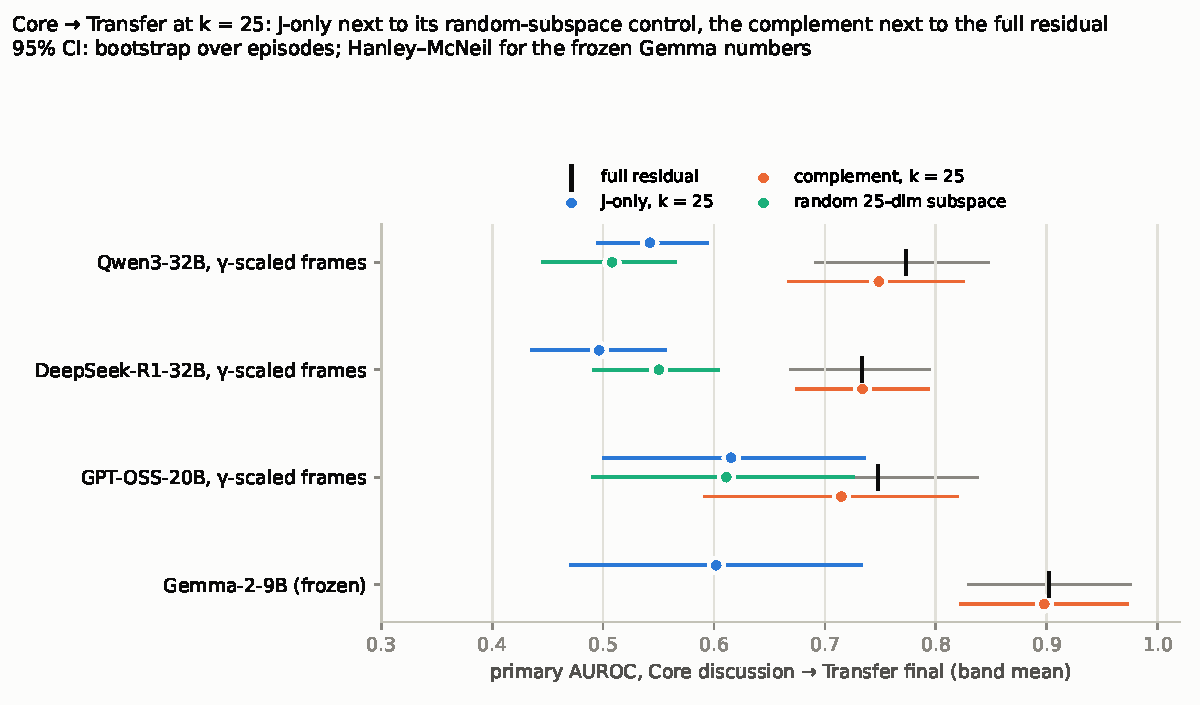
\includegraphics[width=0.95\textwidth]{figures/fig_k25_cross_model_e1.pdf}
\caption{E1: the same comparison as Figure~\ref{fig:cross} with frames chosen from the final-norm-scaled dictionary $\WU\,\mathrm{diag}(\gamma)$.}
\end{figure}

\bibliographystyle{plainnat}
\bibliography{refs}

\end{document}
